% \glsresetall
\chapter{Presentation of the results} % Main chapter title
\label{Chapter6}

\lhead{Chapter 6. \emph{Presentation of the results}}

In this chapter it will be explained how empirical traffic data was gathered using the prototype and which metrics where defined for comparison.
Afterwards the landscapes will be compared using the defined metrics as key performance indicators. The actual evaluation of the results will be concluded in the following chapter.

\section{Data collection and metric definition} 

This section will contain information about how the data was collected and which metrics were defined based on the gathered data.

\subsection{Data collection}

Since multiple landscapes were implemented a unified process was required to collect comparable data. The following BPMN diagram contains the process steps in detail.

\begin{figure}[!h]
	\centering
	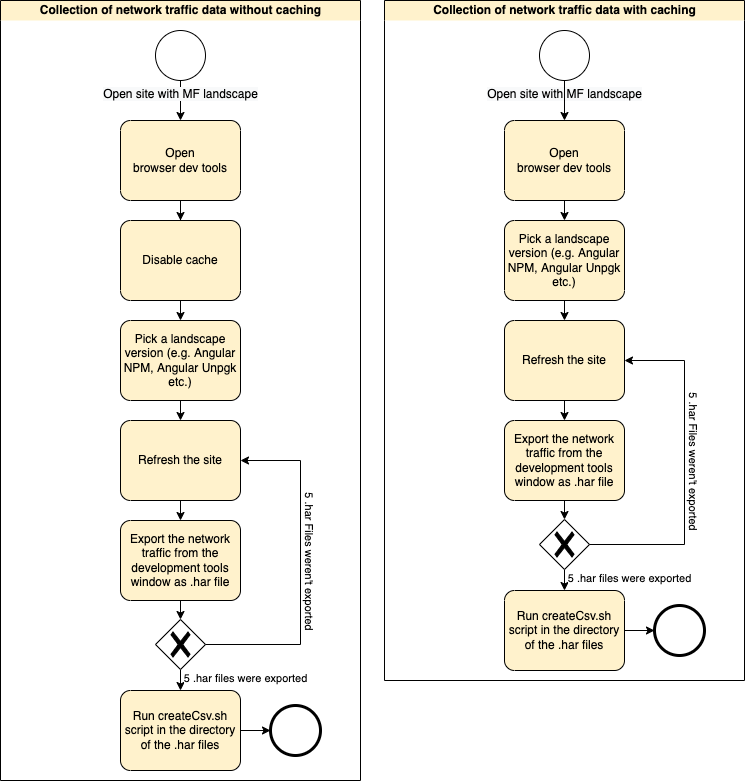
\includegraphics[width=0.7\textwidth]{Figures/Data_Collection_Process_har.drawio.png}
	\caption{Data collection process for .har files}
	\label{fig:data_collection_process_har}
\end{figure}

As it can be seen in \ref{fig:data_collection_process_har} there are actually two processes executed to collect data. The first one were with caching disabled, the second had it enabled. The intention behind it was to gather an average initial loading time for the picked side, therefore the resources must not be cached. 
The second process were used to gather information about caching behavior in general. Since each landscape contains basically the same views, the browser should be able to pull already loaded resources from the cache instead via the network. To showcase this behavior and prove the performance gain through caching this data was gather too.
Each process was executed 5 times, therefore 10 HTTP Archive (\texttt{.har}) files were generated per landscape. These \texttt{.har} files were then transformed into \texttt{.csv} files using a self developed script. 

Additionally to the \texttt{.har} files a website performance report was collected, using the Lighthouse tool embedded in the Google Chrome browser. This report provides information about how much of the imported bytes were actually used by the web application, distinguished by the resources URL.

Following that description following files were generated.

After all data was collected, another self developed script was used to create a central file aggregating all the gather data in a single file. This was later used to define and calculate the metrics, which are described below.

\subsection{Defined metrics}

The central file containing all the data, was split into separate sheets in which the metrics for each micro frontend were calculated. The parameters for calculation were the following.

\begin{itemize}
	\item \textbf{connection} - This is an ID with which each opened TCP connection is tagged by the browser. This value can be an indicator for the parallelity of the requests. Since HTTP/2 several requests can be handled by a server via the same TCP connection, reducing the time costs for TCP handshakes. It has to be considered that the application requesting the sources can not implement this HTTP/2 feature. It has to be enabled on server side and by the browser, which is already the case for most popular browsers.\cite{http2} As of writing this transcript, Surge the web server platform, onto which the application landscapes are deployed, does not support HTTP/2.
	
	\item \textbf{loadedFromCache} - This is string value with three possible characteristics, \textit{not loaded from cache, disk, memory}. Whereas \textit{disk and memory} are semantically the same. This values explains from where the resource was loaded, either via the network from a remote server or from the local cache. This value helps indicating the caching behavior of bundled resources in comparison with resources loaded from a unified URL (e.g. a CDN). 
	
	\item \textbf{pageRef} - This is a page reference provided by the browser with a possibly infinite amount of characteristics. Each request is tagged with this value, so it can be distinguished, which request was sent by which web application. Since the data is separated by sheets inside the file and is always website specific, no further information can be pulled from this value.
	
	\item \textbf{startedDateTime} - This is time stamp given to each request, marking its starting time in a date time format. This value can also an indicator for parallelity since multiple TCP can be opened at the same time. 
	
	\item \textbf{requestMethod}	- This is a string value with a limited amount of characteristics. The possible values are the different HTTP methods. It indicates which type of requests were executed for the loaded resource. In almost all cases it's \textbf{GET}.
	
	\item \textbf{requestUrl} - This is a string value, contain the request URL used by the browser to load the resource. This value is mainly categorizing the calculations results. Since neither \textit{connection} nor \textit{pageRef} are valid options to distinguish the loaded a resources of the web site. 
	
	\item \textbf{requestHeaderSize}	- This is a number value, indicating the byte size in kilobyte of the request header sent by the web application to the server.
	
	\item \textbf{responseStatus} - This is a number value with a limited amount of characteristics, containing the HTTP response code from the server. The range if the possible values is the same as the possible response code of the HTTP.
	
	\item \textbf{responseContentSize} - This number value is byte size of the loaded resource in kilo bytes.
	
	\item \textbf{timeInMs} - This value represents the round trip of the request in milliseconds. 
\end{itemize}

Based on the given values from the \texttt{.har} files, following key performance indicators were calculated.

\begin{itemize}
	\item \textbf{Avg. ContentSize in KB} 
	\item \textbf{Avg Time in MS Loaded values}
	\item \textbf{Occurences Connection Duplicates}
	\item \textbf{Connection Ids Connection IDs occurence}
	\item \textbf{Parallel start time}
	\item \textbf{Avg. Response Time per Connection ID in MS}
	\item \textbf{Avg. Response content size per Loading Type in KB	URLs loaded}
	\item \textbf{Avg. Response Time per URL loaded in MS}
	\item \textbf{Avg. Response Size per URL loaded in KB}
	\item \textbf{Avg. Response Size per URL loaded in KB}
	\item \textbf{Avg. Response Size per URL loaded from Disk in KB}
	\item \textbf{Avg. Response Size per URL loaded from Memory in KB}
\end{itemize}

\section{CDN Implementation}

\section{Web Component Implementation}

\section{WMF Implementation}

\section{Comparison}



